\chapter{Java 技术概述及开发环境}
\label{chp:Introduction-to-Java}

\section*{基本信息}
\sline
\begin{description}
\item[课程名称:] Java应用与开发
\item[授课教师:] 王晓东
\item[授课时间:] 第一周
\item[参考教材:] 本课程参考教材及资料如下:
  \begin{itemize}
  \item 陈国君主编,Java程序设计基础(第5版),清华大学出版社,2015.5
  \item Bruce Eckel, Thinking in Java (3rd)
  \end{itemize}
\end{description}

\section*{教学目标}

\sline
\begin{enumerate}
\item 讲解Java的发展历程,从Java的视角回顾OOP;
\item 理解Java平台的相关概念和机制;
\item 掌握基本的Java开发环境配置方法。
\end{enumerate}  

\section*{授课方式}

\sline
\begin{description}
\item[理论课:] 多媒体教学、程序演示
\item[实验课:] 上机编程
\end{description}

\newpage
\section*{教学内容}
\sline

\section{Java技术概述}

\subsection{Java发展简史}

Java的发展过程中伴随着多个伟大公司的起起落落。

\begin{description}
\item[\fbox{1982}] Sun公司成立(安迪$\cdot$贝托谢姆和麦克尼利)。
\item[\fbox{1986}] Sun公司上市。
\item[\fbox{1985}] Sun公司推出著名的Java语言。
\item[\fbox{2001}] 9.11事件前,Sun市值超过1000亿美元;此后,由于互联网泡沫的破碎,其市值
  在一个月内跌幅超过90\%。
\item[\fbox{2004}] Sun公司和微软在旷日持久的Java官司中和解,后者支付前者高达10亿美元的
  补偿费。
\item[\fbox{2006}] 共同创始人麦克尼利辞去CEO一职,舒瓦茨担任CEO后尝试将Sun从设备公司向软
  件服务型公司转型,但不成功。
\item[\fbox{2010}] Sun公司被甲骨文公司收购。
\end{description}

Java语言的版本迭代历程如图\ref{fig:java-versions}所示。

\begin{figure}[htb]
\centering
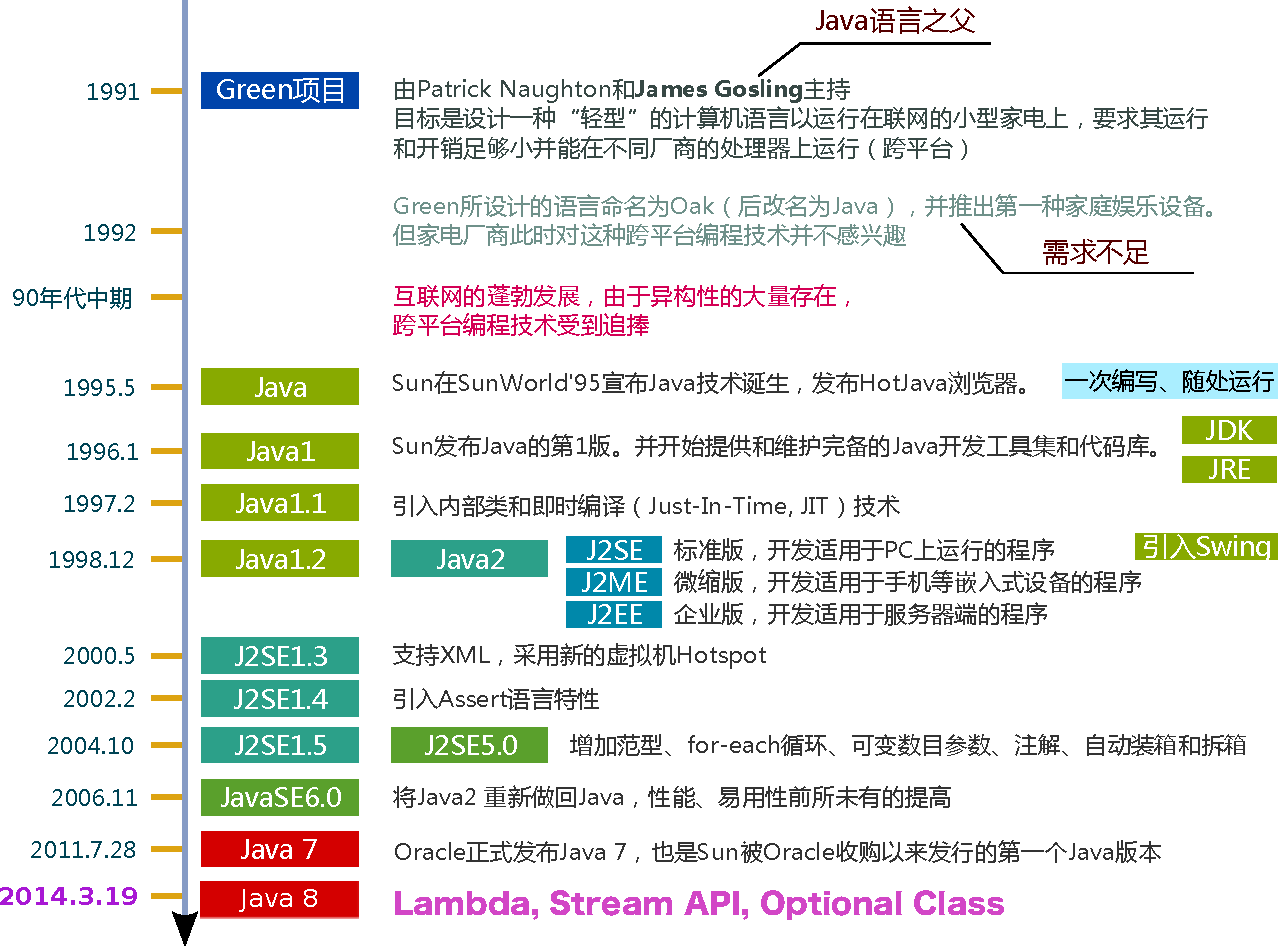
\includegraphics[width=\textwidth]{images/Introduction-to-Java/fig-java-versions.pdf}
\caption{Java版本迭代}
\label{fig:java-versions}
\end{figure}

\subsection{Java技术的特点}

Java具备以下技术特点:

\begin{description}
\item[面向对象] Java是一种以对象为中心,以消息为驱动的面向对象的编程语
  言。
\item[平台无关性] 分为源代码级(需重新编译源代码,如C/C++)和目标代码
  级(Java)平台无关。
\item[分布式] 可支持分布式技术及平台开发。
\item[可靠性] 不支持直接操作指针,避免了对内存的非法访问;自动单元回收
  功能防止内存丢失等动态内存分配导致的问题;解释器运行时实施检查,可发
  现数组和字符串访问的越界;提供了异常处理机制。
\item[多线程] C++没有内置的多线程机制,需调用操作系统的多线程功能来进行
  多线程序设计;Java提供了多线程支持。
\item[网络编程] Java具有丰富的网络编程库。
\item[编译和解释并存] 由编译器将Java源程序编译成字节码文件,再由运行系
  统解释执行字节码文件(解释器将字节码再翻译成二进制码运行)。
\end{description}

\section{Java平台核心机制}


Java技术栈如图\ref{fig:java-tech-stack}所示,程序的编译运行过程如
图\ref{fig:java-running-process}所示。需要了解以下几个核心概念:

\begin{itemize}
\item Java虚拟机
\item 垃圾回收机制
\item Java运行时环境(Java Runtime Environment, JRE)
\item JIT, Just-In-Time 传统解释器的解释执行是转换一条,运行完后就将其扔掉;
  JIT会自动检测指令的运行情况,并将使用频率高(如循环运行)的指令解释后保存下来,下次调用
  时就无需再解释(相当于局部的编译执行),显著提高了Java的运行效率。
\end{itemize}

\begin{figure}[htb]
  \begin{minipage}[t]{0.4\linewidth}
    \centering
    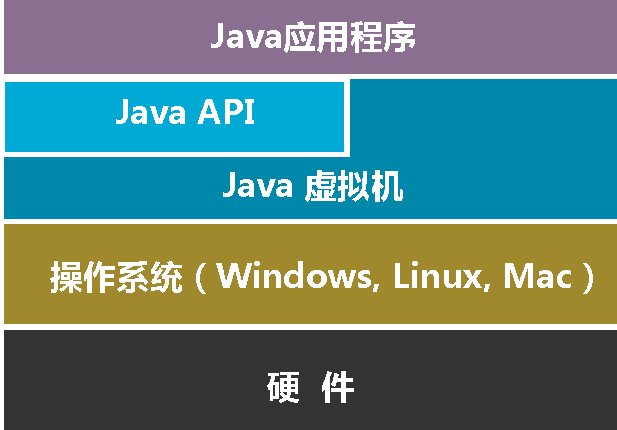
\includegraphics[width=0.9\textwidth]{images/Introduction-to-Java/fig-java-tech-stack.pdf}
    \caption{Java技术栈}
    \label{fig:java-tech-stack}
  \end{minipage}
  \begin{minipage}[t]{0.6\linewidth}
    \centering
    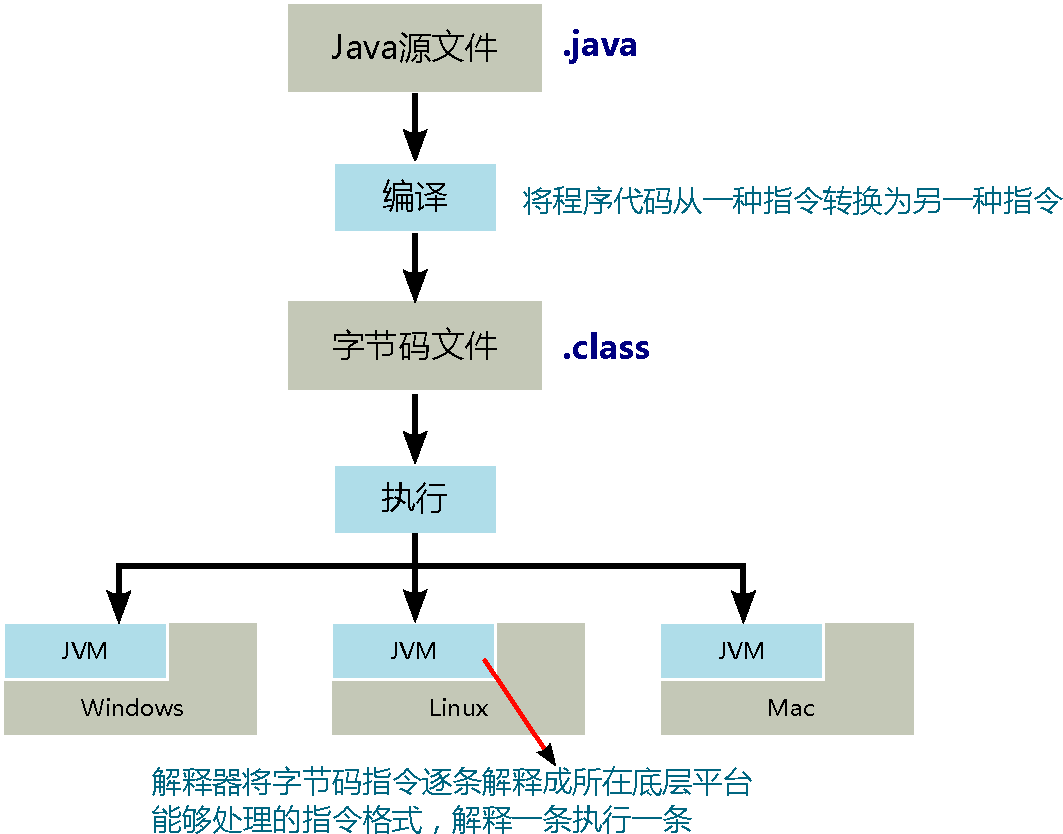
\includegraphics[width=\textwidth]{images/Introduction-to-Java/fig-java-running-process.pdf}
    \caption{Java程序编译运行过程}
    \label{fig:java-running-process}
  \end{minipage}
\end{figure}

\section{Java开发环境}
构建Java开发环境,需要首先获取和安装Java开发工具集,可以从Oracle官方网
站链
接http://www.oracle.com/technetwork/java/javase/downloads/index.html获
取。下载完成后解压放入合适的磁盘目录下。

对于Windows操作系统,可以采用以下路径:

\begin{shCode}
  D:\Program Files\Java
\end{shCode}

对于Linux操作系统,可以采用以下路径:

\begin{shCode}
  /opt/jdk1.8.0_172
\end{shCode}

接下来进行环境变量配置,以Windows操作系统为例:

\begin{description}
\item[\fbox{变量名}] Path
\item[\fbox{变量值}] D:\textbackslash Program Files\textbackslash Java\textbackslash
  jdk1.8.0\_172\textbackslash bin
\end{description}

配置完成后,可以看到JDK目录中包含以下子目录和文件:

\begin{shCode}
  bin  COPYRIGHT  db  include  javafx-src.zip
  jre  lib  LICENSE  man  README.html  release  src.zip
  THIRDPARTYLICENSEREADME-JAVAFX.txt  THIRDPARTYLICENSEREADME.txt  
\end{shCode}

对子目录的功能简要描述如下:

\begin{description}
\item[bin] Java开发工具,包括编译器、虚拟机、调试器、反编译器等;
\item[jre] Java运行时,包括Java虚拟机、类库和其他资源文件;
\item[lib] 类库和所需支持性文件;
\item[include] 用于调试本地方法(底层平台)的C++头文件;
\item[src.zip] 类库的源代码;
\item[db] Java DB数据库,JDK6.0新增项目,一种纯Java的关系型数据库。
\end{description}

\section{Java开发工具}

业界普遍采用Eclipse或IntelliJ IDEA等集成开发环境进行Java大型工程开发,
当然也可以采用文本编程工具Vim或Emacs等进行Java小型程序的开发。

本课程采用Eclipse作为首选集成开发环境。

\section{Java基本开发流程}

本部分使用文本编程工具编写一个简单的Java Hello World程序,演示Java的基
本开发和代码编译运行流程。首先,我们需要使用文本编程工具编写一个Java源
文件HelloWorld.java,文件命名必须与类名相同。

\begin{javaCode}
public class HelloWorld {
    public static void main(String[] args) {
	System.out.println("Hi, Java!");
    }
}   
\end{javaCode}

然后,使用javac工具将源文件编译为字节码文件,编译完成后,我们可以看到生成了HelloWord.class这一字节码文件。

\begin{shCode}
  > javac HelloWorld.java && ls 
  HelloWorld.class  HelloWorld.java
\end{shCode}

接下来,我们使用java工具运行该程序,在终端正确打印了“Hi, Java”字符串。

\begin{shCode}
  > java HelloWorld 
  Hi, Java!
\end{shCode}


\descript{说明}

编写Java应用程序需掌握的几条规则如下:

\begin{enumerate}
\item Java语言拼写是大小写敏感的(Case-Sensitive);
\item 一个源文件中可以定义多个Java类,但其中最多只能有一个类被定义为Public类;
\item 如果源文件中包含了public类,则源文件必须和该public类同名;
\item 一个源文件包含多个Java类时,编译后会生成多个字节码文件,即每个类都会生成一个单独的
  “.class”文件,且文件名与类名相同。
\end{enumerate}

